\section{Process and Results}

\subsection{Capital Asset Pricing Model}

1. Determine the Risk-Free Rate (\(R_f\))

The risk-free rate is typically the return on government bonds, such as U.S. Treasury bills. We decided to use the average risk-free rate over our analysis period for CBOE Interest Rate 10 Year T No \cite{YahooFinanceTNX}

2. Calculate the Expected Market Return (\(R_m\))

The expected market return can be the average return of a broad cryptocurrency market index. For this instance, we used the Bitwise 10 Crypto Index Fund (BITW) \cite{bitw}.

3. Calculate the Beta (\(\beta\))

Beta measures the volatility of a cryptocurrency relative to the market. 

To calculate beta:

\begin{itemize}
    \item Collect Historical Price Data: Obtain historical daily prices for each cryptocurrency and the chosen market index.
    \item Calculate Returns: Compute the daily returns for each cryptocurrency and the market index.
    \item Run a Regression Analysis: Perform a linear regression with the cryptocurrency returns as the dependent variable and the market index returns as the independent variable. The slope of the regression line is the beta.
\end{itemize}

4. Compute the Market Risk Premium (\(R_m - R_f\))

The market risk premium is the difference between the expected market return and the risk-free rate.

\begin{table}[h]
\centering
\begin{tabular}{|c|c|c|c|}
\hline
\textbf{Asset} & \textbf{Beta} & \textbf{Market Risk Premium} & \textbf{Expected Return (CAPM)} \\
\hline
AAPL & 0.1489 & -0.0346 & 0.0294 \\
MSFT & 0.1469 & -0.0346 & 0.0295 \\
AMZN & 0.2194 & -0.0346 & 0.0270 \\
GOOGL & 0.1653 & -0.0346 & 0.0289 \\
TSLA & 0.2734 & -0.0346 & 0.0251 \\
SPY & 0.1084 & -0.0346 & 0.0308 \\
DJI & 0.0089 & -0.0346 & 0.0343 \\
AGG & 0.0115 & -0.0346 & 0.0342 \\
VNQ & 0.0884 & -0.0346 & 0.0315 \\
GLD & 0.0195 & -0.0346 & 0.0339 \\
USO & 0.0408 & -0.0346 & 0.0332 \\
SLV & 0.0671 & -0.0346 & 0.0323 \\
PSP & 0.1596 & -0.0346 & 0.0291 \\
BTC-USD & 0.4680 & -0.0346 & 0.0184 \\
ETH-USD & 0.5448 & -0.0346 & 0.0157 \\
SOL-USD & 0.7253 & -0.0346 & 0.0095 \\
BNB-USD & 0.3944 & -0.0346 & 0.0209 \\
XRP-USD & 0.5699 & -0.0346 & 0.0149 \\
TON-USD & 0.4154 & -0.0346 & 0.0202 \\
DOGE-USD & 0.4995 & -0.0346 & 0.0173 \\
ADA-USD & 0.5541 & -0.0346 & 0.0154 \\
SHIB-USD & 0.5231 & -0.0346 & 0.0165 \\
AVAX-USD & 0.6062 & -0.0346 & 0.0136 \\
\hline
\end{tabular}
\caption{CAPM Estimates for Various Assets}
\label{tab:capm}
\end{table}


More information can be found in appendix, please refer to \ref{appendix:capm_details}.


\begin{figure}
    \centering
    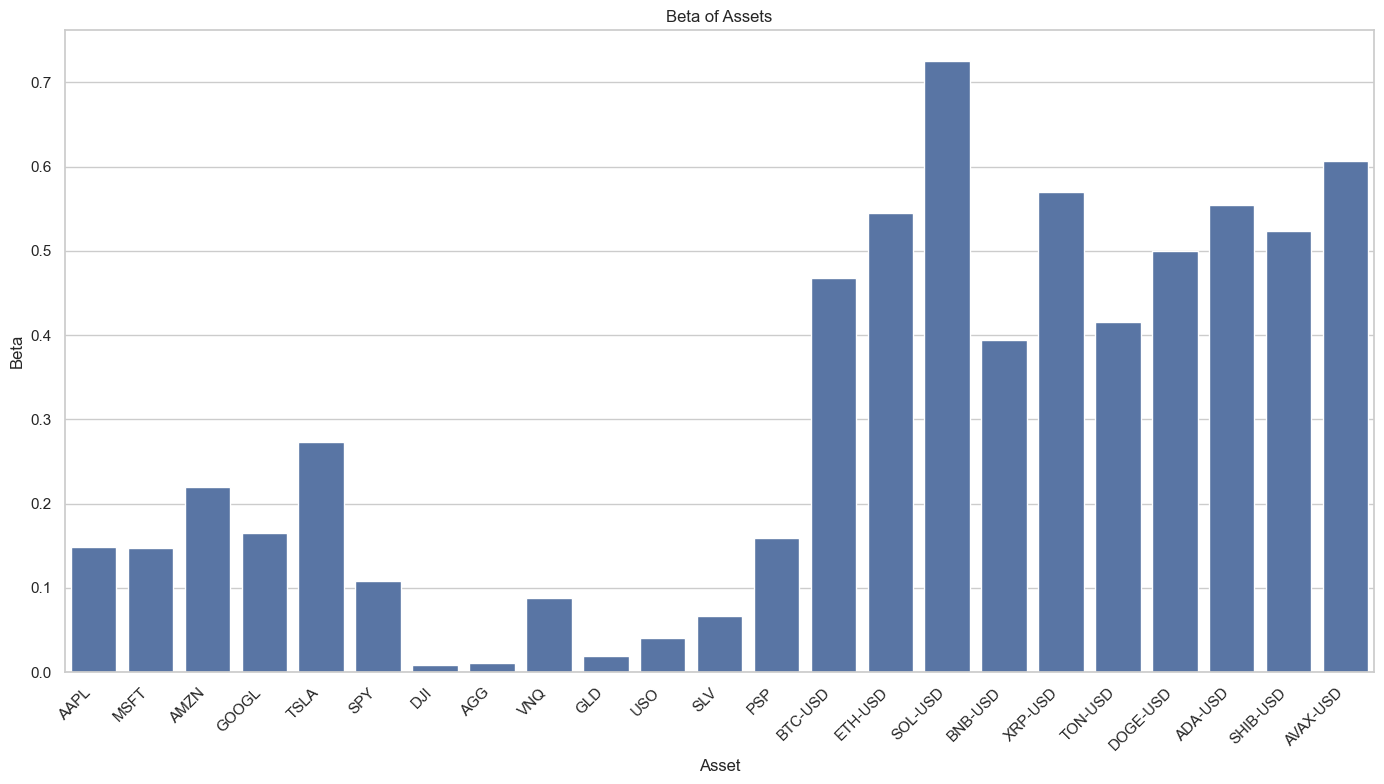
\includegraphics[width=0.8\textwidth]{./code/risk-and-return-analysis/capm/beta_assets.png}
    \caption{Beta of Cryptocurrencies Relative to BITW}
    \label{fig:beta}
\end{figure}

\begin{figure}
    \centering
    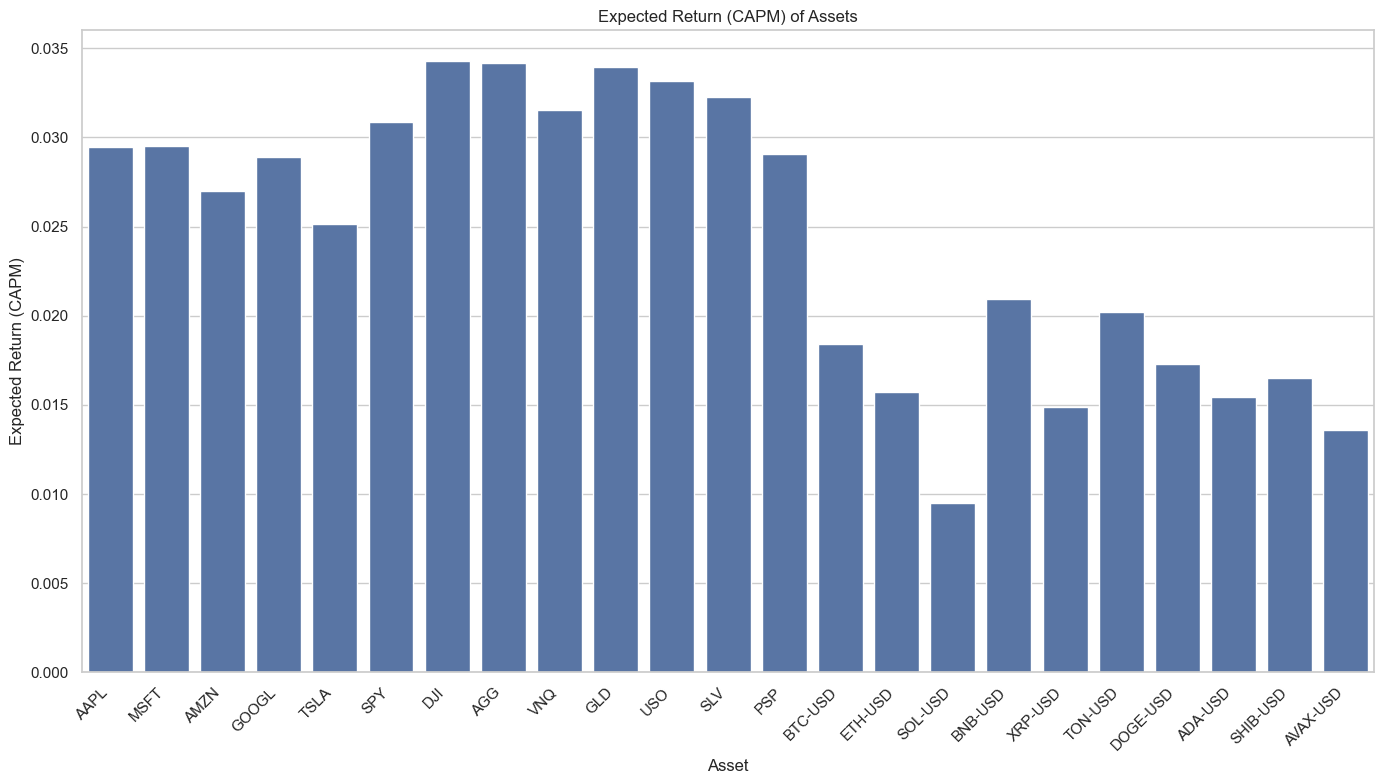
\includegraphics[width=0.8\textwidth]{./code/risk-and-return-analysis/capm/exp_return_assets.png}
    \caption{Expected Return of Cryptocurrencies Relative to BITW}
    \label{fig:exp_return}
\end{figure}